The Density Matrix Renormalization Group (DMRG) algorithm, which was subsequently understood as a variational method over the class of Matrix Product States (MPS), has developed to be the de-facto standard for the numerical simulation of one-dimensional quantum systems. The success of this method is due to the remarkable ability of MPS to capture the area-law entanglement characteristics of ground states of gapped Hamiltonians. Additionally, due to the elegant diagrammatic notation for tensor networks, new algorithms can be developed and discussed efficiently and intuitively. Applications of MPS include finding ground and thermal states, real and imaginary time evolution, and the computation of dynamical properties of lattice Hamiltonians. In the following we give a brief introduction to MPS, for a more in-depth discussion see \cite{cite:DMRG_in_the_age_of_MPS, cite:practical_introduction_MPS_and_PEPS, cite:tenpy}. \par
The state of a quantum many-body system can be written as
\begin{equation}
	\left|\Psi\right\rangle = \sum_{i_1=1}^{d_1} \sum_{i_2=1}^{d_2} \cdots \sum_{i_N=1}^{d_N} \Psi_{i_1i_2\dots i_N} \left|i_1\right\rangle \otimes \left|i_2\right\rangle \otimes \cdots \otimes \left|i_N\right\rangle.
\end{equation}
where N is the number of subsystems (e.g. lattice sites or particles), and $\left\{\left|i_1\right\rangle \otimes \left|i_2\right\rangle \otimes \dots \otimes \left|i_N\right\rangle\right\}$, $i_j = 0, \dots, d_j$ is a set of basis vectors of the full many-body Hilbert space
\begin{equation}
	\mathcal{H} = \bigotimes_{j=1}^{N} \mathcal{H}_j,
\end{equation}
with $\dim\left(\mathcal{H}_j\right) = d_j$ the dimension of the local Hilbert space of subsystem $j$. To simplify the notation, we will assume that the dimension of all local subsystems is the same, $d_j = d$. The $d^N$ complex numbers $\Psi_{i_1i_2\dots i_N}$ fully describe the quantum many-body state, and one can think of $\Psi\in\mathbb{C}^{d\times\cdots\times d}$ as a tensor of rank $N$. However, due to the size of the tensor scaling exponentially with system size, only very small system sizes are accessible computationally. One proceeds by writing $\Psi$ as a tensor network of smaller tensors. A \textit{Matrix Product State} (MPS) is constructed by introducing $N$ rank-3 tensors $A^{[n]}\in\mathbb{C}^{d\times \chi_{n-1}\times \chi_{n}}$ and contracting them in a chain as
\begin{equation}
	\label{eq:MPS_open_boundary_conditions_general_definition}
	\Psi_{i_1i_2\cdots i_N} \coloneqq \sum_{\alpha_1=1}^{\chi_1} \sum_{\alpha_2=1}^{\chi_2}\dots\sum_{\alpha_{N-1}=1}^{\chi_{N-1}}A^{[1],i_1}_{1,\alpha_1} A^{[1],i_2}_{\alpha_1,\alpha_2} \cdots A^{[N],i_N}_{\alpha_{N-1},1},
\end{equation}
where we have written the physical indices $i_n$ as superscripts, such that the sums are performed only over subscripts. Note that in this notation the bond dimensions at the two ends of the chain is $\chi_0 = \chi_{N} = 1$, and we can interpret the tensors $A^{[1]}$ and $A^{[N]}$ as tensors of rank-2. A tensor diagram of the MPS \eqref{eq:MPS_open_boundary_conditions_general_definition} is given in figure \figref{fig:mps_general}.\par
\begin{figure}
	\centering
	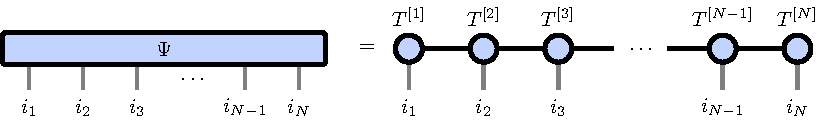
\includegraphics[scale=1]{figures/tikz/Tensor_Networks/mps_basic/mps_basic.pdf}
	\caption{Diagrammatic representation of the Matrix Product State \ref{eq:MPS_open_boundary_conditions_general_definition}.}
	\label{fig:mps_general}
\end{figure}
\begin{figure}
	\centering
	\subcaptionbox{\label{fig:mps_canonical_form_general_definition}}
	{%
		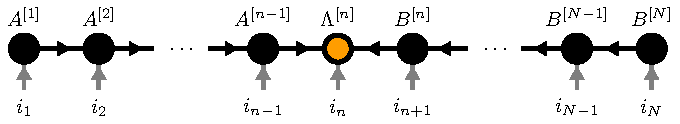
\includegraphics[scale=1]{figures/tikz/Tensor_Networks/mps_canonical_form/mps_canonical_form_a.pdf}
	}
	\subcaptionbox{\label{fig:mps_left_isometry_condition}}
	{%
		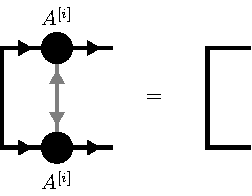
\includegraphics[scale=1]{figures/tikz/Tensor_Networks/mps_canonical_form/mps_canonical_form_b.pdf}
	}
	\quad\quad\quad\quad\quad\quad
	\subcaptionbox{\label{fig:mps_right_isometry_condition}}
	{%
		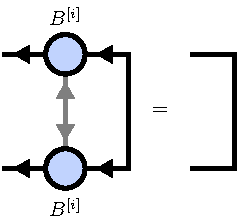
\includegraphics[scale=1]{figures/tikz/Tensor_Networks/mps_canonical_form/mps_canonical_form_c.pdf}
	}
	\caption{(a) Diagrammatic representation of an MPS in canonical form. (b) The left isometry condition. (c) The right isometry condition.}
	\label{fig:mps_canonical}
\end{figure}
An important property of MPS is the existence of a \textit{canonical form} as an isometric tensor network, where a single tensor $A^{[n]}$ is selected as the orthogonality center. One can bring an arbitrary MPS into this canonical form through successive QR-decompositions or SVDs, starting at the outer ends of the chain and isometrizing one tensor at a time, until the orthogonality center is reached \cite{cite:DMRG_in_the_age_of_MPS}. In figure \figref{fig:mps_canonical_form_general_definition} an MPS in canonical with the orthogonality center at subsystem $n$ is visualized in diagrammatic notation. The canonical form greatly simplifies many operations on MPS and allows for the formulation of efficient algorithms, where many contractions reduce to identity due to the isometry condition \eqref{eq:isometry_condition_general}, see also figure \figref{fig:mps_left_isometry_condition} and \figref{fig:mps_right_isometry_condition}. For example, the expectation value $\left\langle\Psi\right|\hat{O}\left|\Psi\right\rangle$ of a one-site operator $\hat{O} \in \mathbb{C}^{d\times d}$ acting on site $n$ can for a general MPS be computed as
\begin{equation}
\begin{split}
	\label{eq:computation_of_expectation_value_MPS}
	\left\langle\Psi\right|\hat{O}\left|\Psi\right\rangle &=\sum_{i_1,\dots,i_N,j_n=1}^{d}\Psi_{i_1,i_2,\dots,i_N} \Psi_{i_1,\dots,i_{n-1},j_n,i_{n+1},\dots,i_N}^* \left\langle j_n\right|\hat{O} \left|i_n\right\rangle \\
	&= \sum_{i_1,\dots,i_N,j_n=1}^{d} \left(A^{[1],i_1}\cdots A^{[N],i_N}\right) \\
	&\quad\quad\quad\quad\quad\,\,\cdot\left(A^{[1],i_1*}\cdots A^{[N],j_n*} \cdots A^{[N],i_N*}\right)\cdot \hat{O}_{i_n,j_n},
\end{split}
\end{equation}
where the $A^{[n],i_n}$ are interpreted as matrices for $1 < n < N$ and as row/column vectors for $n = 1, N$ such that the product
\begin{equation}
	\left(A^{[1],i_1}\cdots A^{[N],i_N}\right)
\end{equation}
gives a scalar. The contraction \eqref{eq:computation_of_expectation_value_MPS} is visualized as a tensor diagram in figure \figref{fig:mps_local_expectation_value}. Here, the advantage of the diagrammatic notation becomes appearant: It is much easier to understand how tensors are contracted when expressing the contraction in terms of tensor network diagrams. The computational cost of computing the expectation value like this scales linear with the system size $\mathcal{O}\left(N\chi^3d\right)$, where $\chi$ is the maximum virtual bond dimension $\chi = \max\left\{\chi_1,\dots,\chi_N\right\}$. If the MPS is however given in canonical form with the orthogonality center at site $n$, the computation reduces to a contraction of only three tensors as can be seen in figure \figref{fig:mps_local_expectation_value_canonical}, and the computational cost $\mathcal{O}\left(\chi^3d\right)$ becomes independent of system size. \par
\begin{figure}
	\centering
	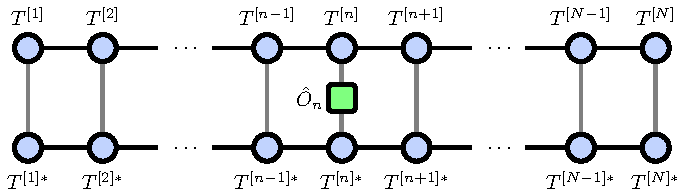
\includegraphics[scale=1]{figures/tikz/Tensor_Networks/mps_local_expectation_value/mps_local_expectation_value.pdf}
	\caption{The computation of the expectation value of a local operator can be computed by contracting the MPS with its conjugate transpose, with the operator "sandwiched" between.}
	\label{fig:mps_local_expectation_value}
\end{figure}
\begin{figure}
	\centering
	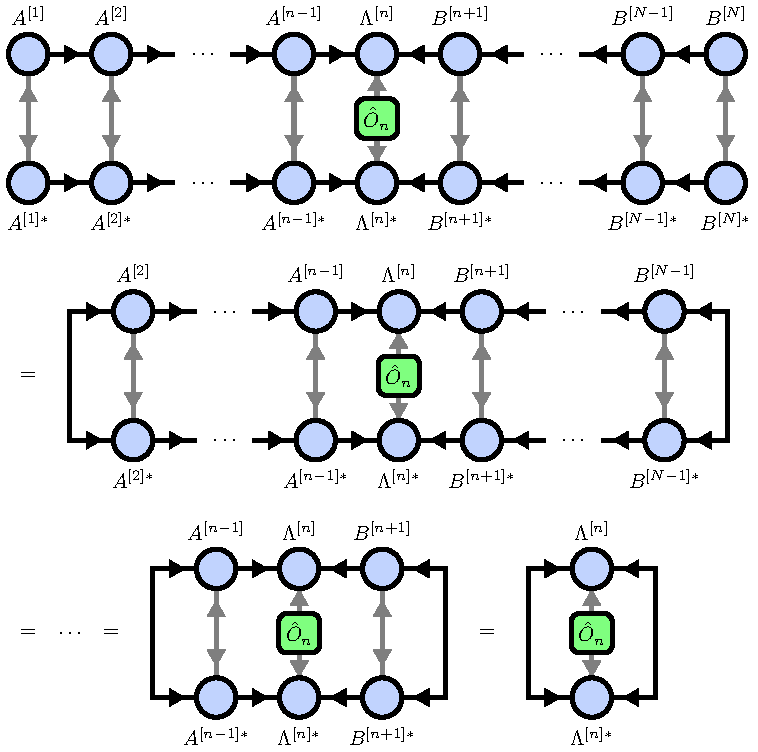
\includegraphics[scale=1.0]{figures/tikz/Tensor_Networks/mps_canonical_form_local_expectation_value/mps_canonical_form_local_expectation_value.pdf}
	\caption{If the MPS is in canonical form, the computation of the expectation value of a local operator can be simplified to a contraction of three tensors using the isometry condition.}
	\label{fig:mps_local_expectation_value_canonical}
\end{figure}
Until now, the MPS representation of $\left|\Psi\right\rangle$ is still exact. One can approximate a MPS by restricting the virtual bond dimension to a maximal bond dimension $\chi_n < \chi_\text{max}$. In this case, the number of parameters that need to be stored to describe the state is reduced from $\mathcal{O}\left(d^N\right)$ to $\mathcal{O}\left(N\chi_\text{max}^2 d\right)$. To arrive at this approximation, two neighbouring tensors can be contracted and split via a truncated SVD, keeping only the $\chi_\text{max}$ largest singular values. If the orthogonality center of the MPS is at one of the two tensors, this approximation is globally optimal as explained in section \ref{sec:tensors_and_tensor_networks_isometric_tensor_networks}. Additionally, this SVD at the orthogonality center is related to the Schimdt decomposition of a bipartite system
\begin{equation}
	\left|\Psi\right\rangle = \sum_{\alpha=1}^{\chi_n} \lambda_\alpha \left| \Psi^{[L]}_\alpha\right\rangle \otimes \left|\Psi^{[R]}_\alpha\right\rangle,
\end{equation}
where the chain is split into a left and right subsystem with orthogonal basis vectors $\left|\Psi^{[L]}_\alpha\right\rangle$ and $\left|\Psi^{[R]}_\alpha\right\rangle$ as visualized in figure \ref{fig}. In this case, the Schmidt values $\lambda_\alpha >= 0$ coincide with the singular values! One can further use this to compute the Von-Neumann entanglement entropy
\begin{equation}
	S = -\sum_{\alpha=1}^{\chi_n} \lambda_\alpha^2 \log\left(\lambda_\alpha^2\right),
\end{equation}
quantifying the amount of entanglement between the left and right subsystems. If the state is normalized, it additionally holds
\begin{equation}
	\sum_{\alpha=1}^{\chi_n} \lambda_\alpha^2 = 1.
\end{equation}
Thus, how well an MPS of a given bond dimension $\chi_\text{max}$ is able to represent a given quantum state is highly dependent on the Schmidt spectrum $\left\{\lambda_\alpha\right\}$ at the different bipartitions of the chain. If the Schmidt values decrease exponentially, only an exponentially small part of the entanglement structure is truncated and the truncated MPS is a good approximation for the original state. It can be shown \cite{cite:area_law_1D_proof, cite:area_laws_review} that for ground states of local, gapped, one dimensional Hamiltonians there holds an \textit{area law}: The entanglement entropy at arbitrary bipartitions of the chain is bounded by a constant
\begin{equation}
	S \le S_\text{max}, 
\end{equation}
where $S_\text{max}$ is independent of the system size. This is in contrast to the fact that the entanglement of states drawn randomly from the many-body Hilbert space on average exhibits \textit{volume law} scaling
\begin{equation}
	\mathbb{E}\left[S\right] > \min\left(N_L, N_R\right)\log(d),
\end{equation}
where $N_L$ and $N_R$ are the number of subsystems in the left and right bipartition. Hence, ground states of gapped Hamiltonians are very nongeneric. Note that the constant $S_\text{max}$ scales with the correlation length of the system, which diverges when approaching critical points. \par
It is immediately clear that truncated MPS by construction exhibit area law entanglement scaling, if the local subsystems that are represented by each tensor correspond to physical systems on a 1D chain. The maximal entanglement entropy for a bipartition can be reached when all Schmidt values are equal, $\lambda_\alpha = 1/\sqrt{\chi_n}$, and thus
\begin{equation}
	S \le \log\left(\chi_\text{max}\right)
\end{equation}
for arbitrary bipartitions of the chain. One can conclude that MPS are good approximations for ground states of gapped 1D Hamiltonians away from criticality. \par 
For completeness we note that the truncation of all bonds of an MPS is a highly non-linear optimization problem and the naive algorithm of truncating each bond with an SVD does in general not lead to a minimal error. A variational compression procedure can often be used to obtain a lower error at the same maximum bond dimension $\chi_\text{max}$ \cite{cite:DMRG_in_the_age_of_MPS}.
\par
Many algorithms have been formulated in the language of MPS. Most notably, the Density Matrix Renormalization Group (DMRG) algorithm can be used for finding ground states of local lattice Hamiltonians \cite{cite:DMRG_in_the_age_of_MPS}. Time evolution of MPS can be performed with the the Time Evolving Block Decimation (TEBD) algorithm \cite{cite:efficient_simulation_of_1D_quantum_many_body_systems, cite:matrix_product_density_operators_simulation_of_finite_temperature_and_dissipative_systems} or the Time Dependant Variational Principle (TDVP) \cite{cite:time_dependent_variational_principle_for_quantum_lattices, cite:unifying_time_evolution_and_optimization_with_MPS}. In the following, we will briefly discuss TEBD, as the algorithm can be generalized easily to isometric tensor product states of higher dimension, which we will do in section \ref{} \todo{Add ref}. \par
Assume that we are given a quantum state $\left|\Psi\right\rangle$ in the form of an MPS and a Hamiltonian $\hat{H}$ that can be written as a sum of nearest-neighbour operators $\hat{h}_{j,j+1}$,
\begin{equation}
	\hat{H} = \sum_{j = 1}^{N-1} \hat{h}^{[j,j+1]}.
\end{equation}
The state $\left|\Psi\right\rangle$ can be evolved in time as
\begin{equation}
	\left|\Psi(t)\right\rangle = \hat{U}\left(t\right) \left|\Psi\right\rangle = e^{-it\hat{H}} \left|\Psi\right\rangle,
\end{equation}
where we set $\hbar = 1$. The time evolution operator $U(t)$ is in general very hard to compute and handle exactly. Thus, $U(t)$ is approximated using a Suzuki-Trotter decomposition. We start by decomposing the time evolution into a series of $K$ small time steps $\Delta t = t/K$ as
\begin{equation}
	U(t) = e^{-it\hat{H}} = \left(e^{-i\Delta t\hat{H}}\right)^K = \left(U(\Delta t)\right)^K.
\end{equation}
Next, we split the Hamiltonian into terms acting on even and odd bonds
\begin{equation}
	\hat{H} = \sum_{j \text{ even}}\hat{h}^{[j, j+1]} + \sum_{j \text{ odd}}\hat{h}^{[j, j+1]} \eqqcolon H_\text{even} + H_\text{odd}.
\end{equation}
Using the Zassenhaus formula
\begin{equation}
	e^{\varepsilon(A+B)} = e^{\varepsilon A} e^{\varepsilon B} e^{-\frac{\varepsilon^2}{2}[A, B]} e^{\frac{\varepsilon^3}{6}\left(2[B,[A,B]]+[A,[A,B]]\right)} \dots
\end{equation}
which can be derived from the Baker-Campbell-Hausdorff formula, we can approximate
\begin{equation}
	\begin{split}
		U(\Delta t) &= e^{-i\Delta t\left(H_\text{even} + H_\text{odd}\right)} = e^{-i\Delta tH_\text{even}}e^{-i\Delta tH_\text{odd}} + \mathcal{O}\left(\Delta t^2\right) \\
		&= \hat{U}^\text{TEBD1}(\Delta t) + \mathcal{O}\left(\Delta t^2\right),
	\end{split}
\end{equation}
which is called a Suzuki-Trotter decomposition of first order. Since operators acting on even bonds commute with each other, the exponentials $e^{-i\Delta tH_\text{even}}$ factorize,
\begin{equation}
	e^{-i\Delta tH_\text{even}} = e^{-i\Delta t\sum_{j \text{ even}} h^{[j, j+1]}} = \prod_{j \text{ even}} e^{-i\Delta t h^{[j, j+1]}},
\end{equation}
and the same is true for the exponentials $e^{-i\Delta tH_\text{odd}}$. Each bond operator $e^{-i\Delta t h^{[j, j+1]}}$ acting on the combined Hilbert space of sites $j$ and $j+1$ can be reshaped into a tensor of rank 4. The application of the operator $\hat{U}^\text{TEBD1}(\Delta t)$ to a state in MPS form can thus be written as the tensor network in figure \figref{fig:mps_tebd_first_order_overview}.
To perform a single TEBD iteration corresponding to a time evolution of $\Delta t$ we want to approximate this tensor network by a new MPS. This can be done by moving the orthogonality center from left to right, applying the bond operators $e^{-i\Delta t h^{[j, j+1]}}$ while keeping the MPS structure. The process of applying a single bond operator is shown in figure \figref{fig:mps_tebd_first_order_applying_bond_op}. First, the two site tensors and $e^{-i\Delta t h^{[j, j+1]}}$  are contracted into a single tensor, that is then split and truncated again using an SVD. By sweeping twice across the MPS, first applying the bond operators on all even bonds and then the bond operators on all odd bonds, we perform a full TEBD iteration. There exist two sources of errors, the truncation error of the truncated SVD and the error of the Suzuki-Trotter decomposition. The truncation error can be controlled by choosing a larger bond dimension $\chi$, allowing the representation of more entanglement and thus the evolution to larger times. However, generally the amount of entanglement grows exponentially in time, necessitating an exponentially growing bond dimension and practically limiting the algorithm to small times. A smaller Suzuki-Trotter error can be achieved by choosing smaller time steps $\Delta t$ or by performing a higher-order Suzuki-Trotter decomposition. For example, a second order decomposition can be computed as
\begin{equation}
	\begin{split}
		U(\Delta t) &= e^{-i\Delta t\left(H_\text{even} + H_\text{odd}\right)} = e^{-i\frac{\Delta t}{2}H_\text{even}} e^{-i\Delta t H_\text{odd}} e^{-i\frac{\Delta t}{2}H_\text{even}} + \mathcal{O}\left(\Delta t^3\right)\\
		&= \hat{U}^\text{TEBD2}(\Delta t) + \mathcal{O}\left(\Delta t^3\right).
	\end{split}
\end{equation}
and can be applied to a MPS similarly as the first order decomposition. For higher order Suzuki-Trotter decompositions see \cite{cite:finding_exponential_product_formulas_of_higher_orders}.
\begin{figure}
	\centering
	\subcaptionbox{\label{fig:mps_tebd_first_order_overview}}
	{%
		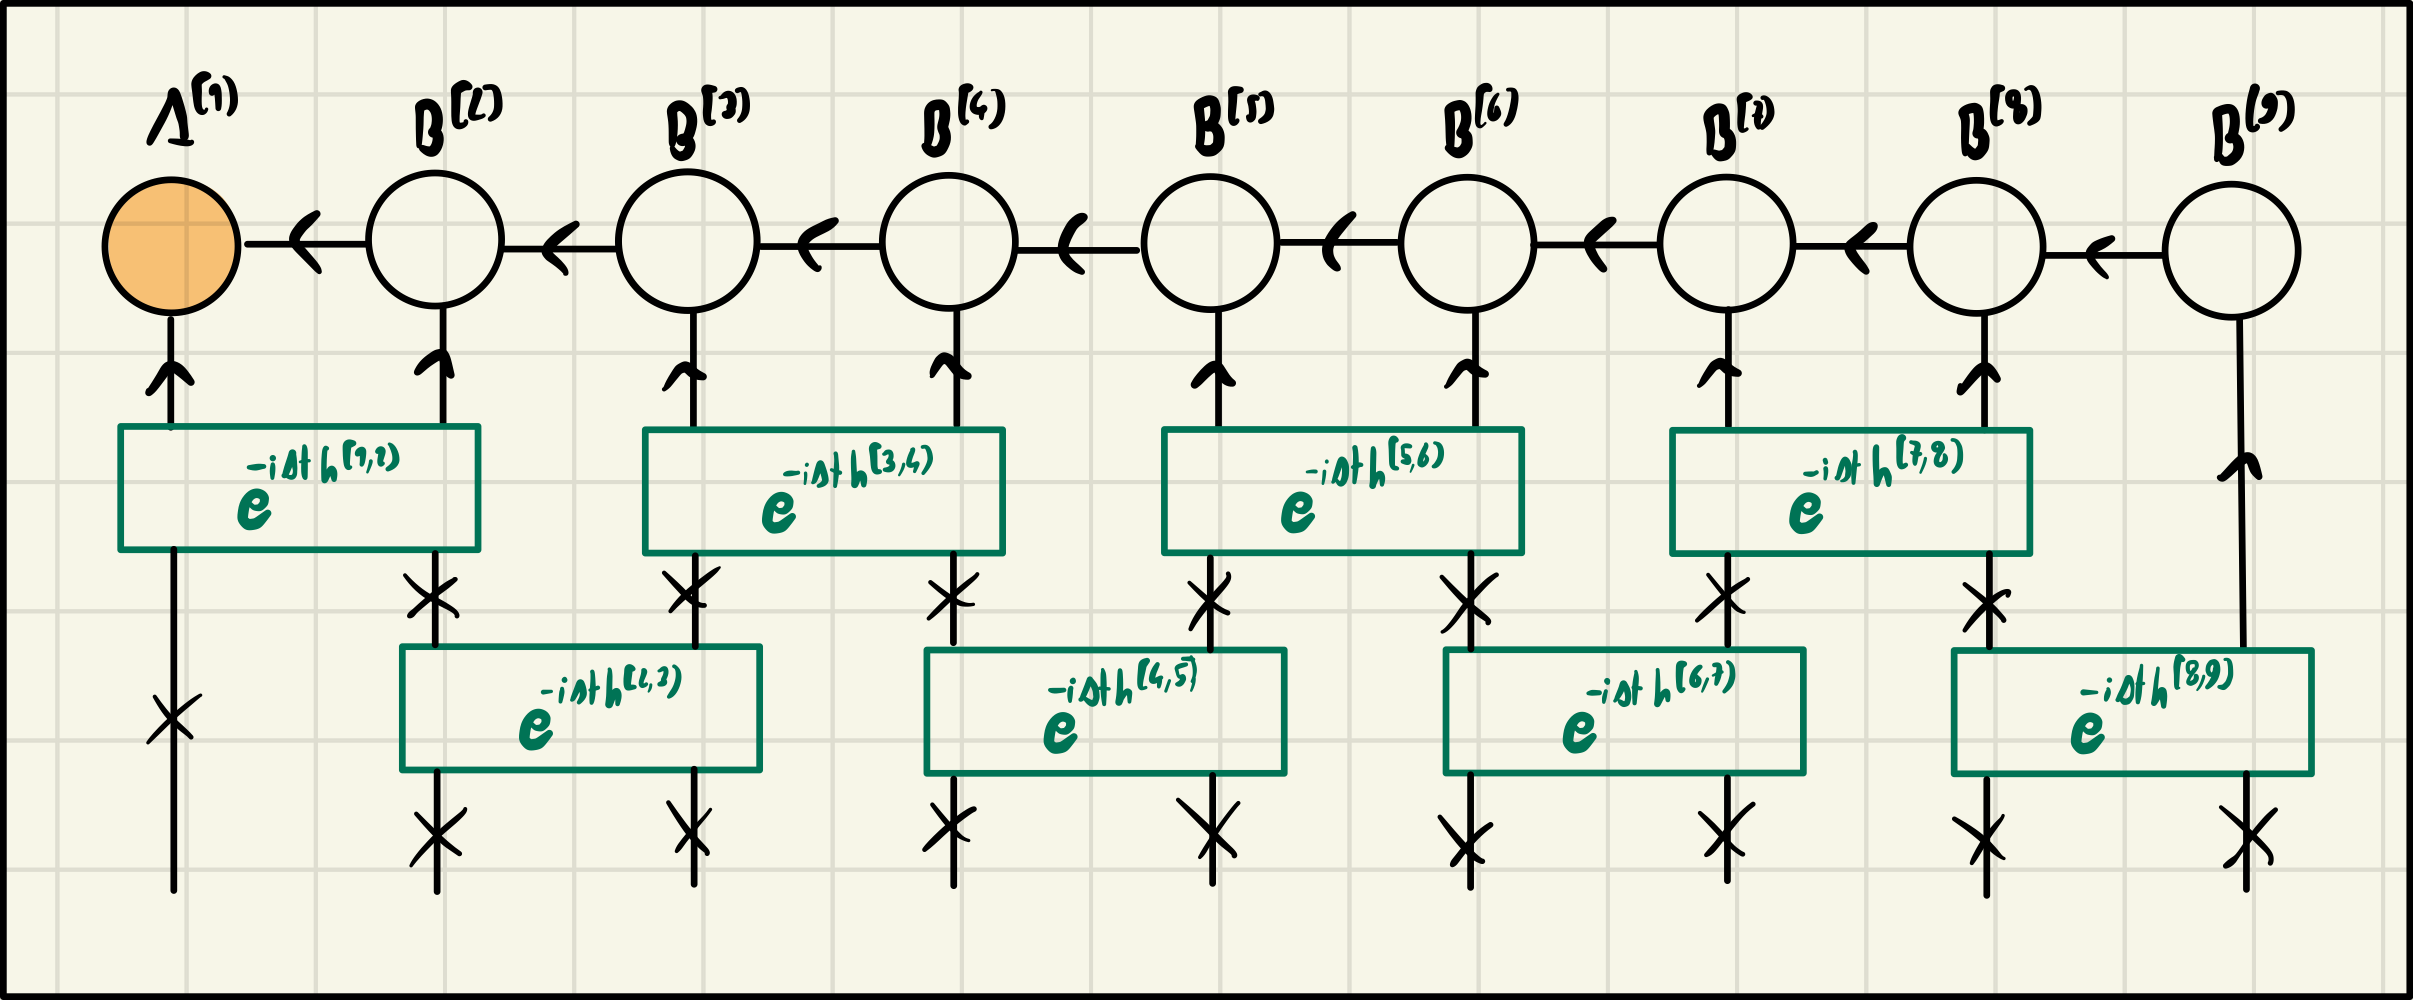
\includegraphics[width=0.8\textwidth]{figures/Tensor_Networks/mps_tebd_first_order.jpeg}
	}
	\subcaptionbox{\label{fig:mps_tebd_first_order_applying_bond_op}}
	{%
		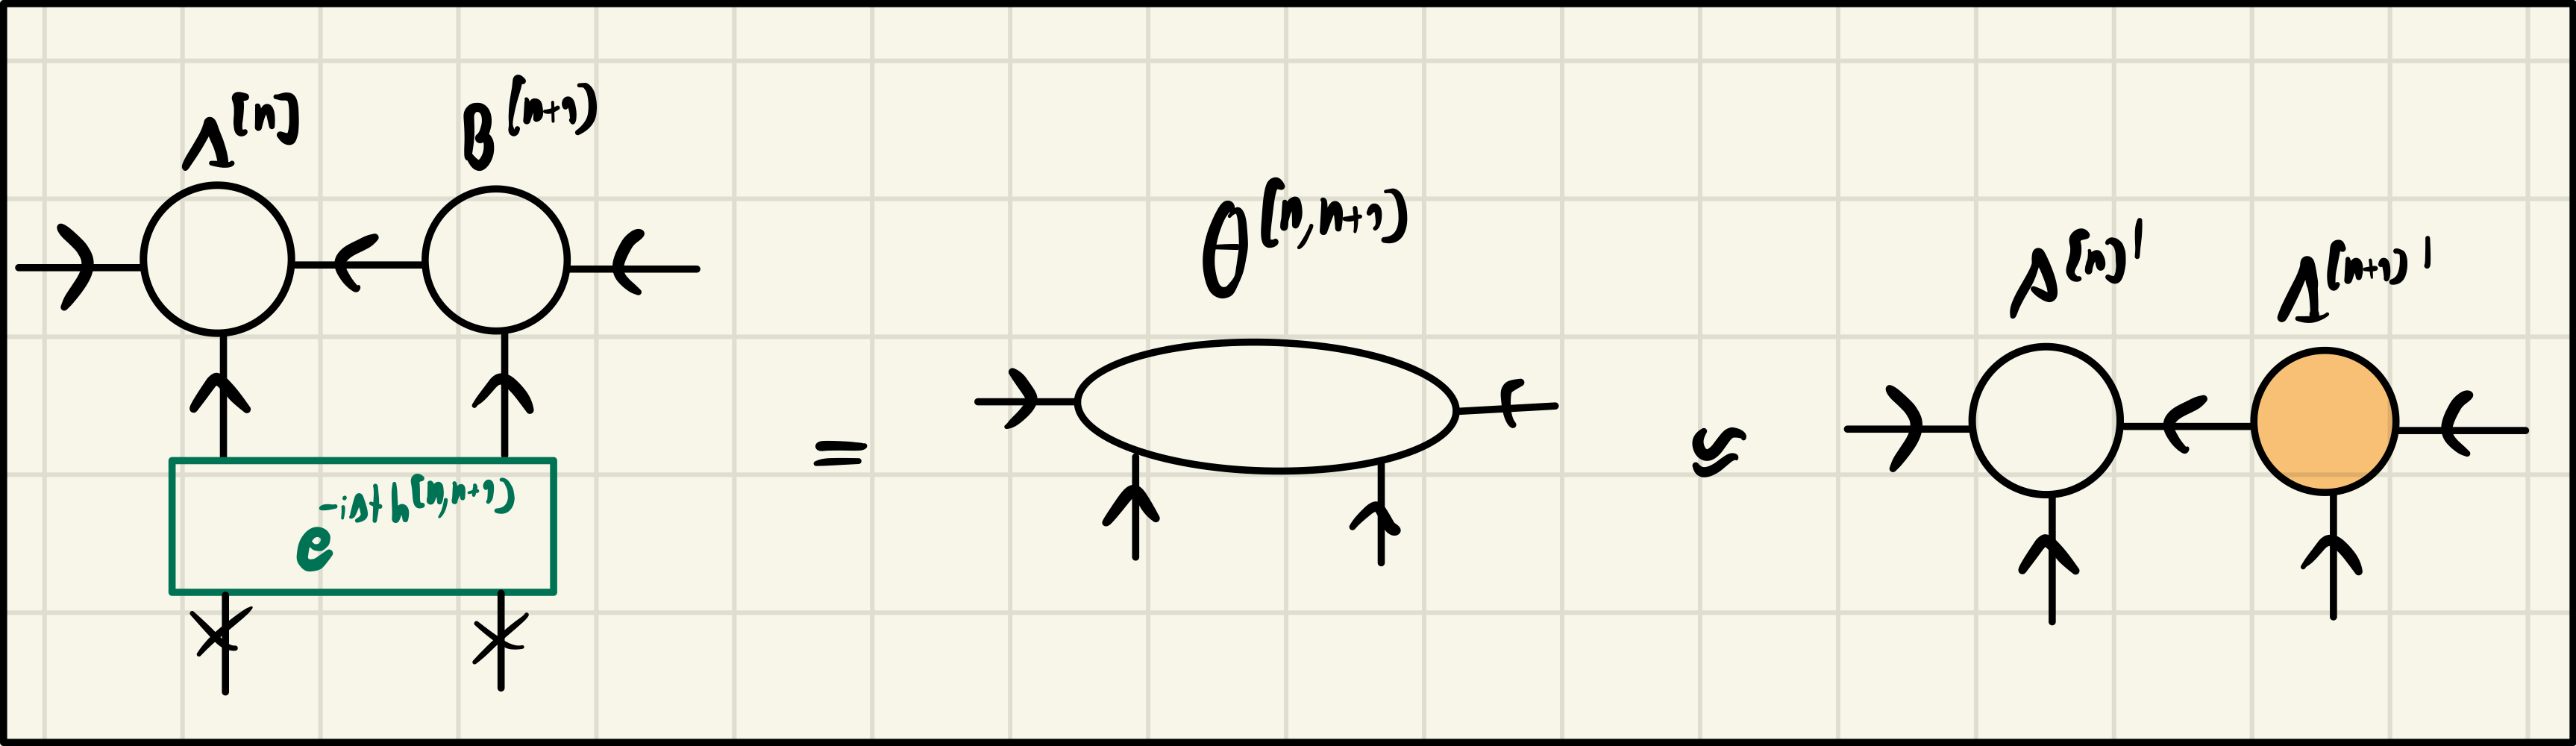
\includegraphics[width=0.8\textwidth]{figures/Tensor_Networks/mps_tebd_applying_bond_op.jpeg}
	}
	\caption{TODO}
	\label{fig:mps_tebd_first_order}
\end{figure}